The purpose of this section is to illustrate the various knowledge representations, depicted in Figure~\ref{fig:ProcessDataFlow}, and the flow from one knowledge representation to the next through a specific example. The description of the flow at each level of the architecture is given in the next subsections.
The example employed in this section uses the operator \textsl{take-kt}, previously mentioned in section~\ref{subsect:Planning_Operators}. \textbf{Description in English coming up...}

\subsection{State Variable Representation}


\subsection{OWL-S Representation}

\begin{figure}[htb]
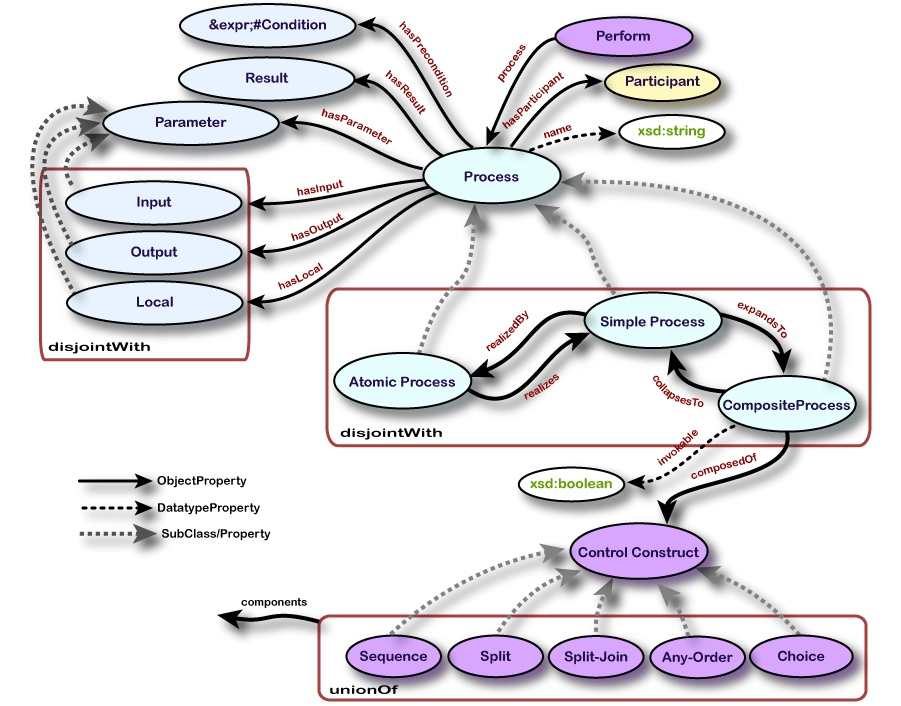
\includegraphics[width=8cm]{images/OWL-S.jpg}
\caption{Selected classes and properties of the profile \cite{OWL-S}.}
\label{fig:OWL-S}
\end{figure}
Once the action is specified in state variable (SV) representation, we can use that information to create an OWL-S process. Figure \ref{fig:OWL-S} shows a schematic of the OWL-S structure. It is outside of the scope of this paper to describe this figure in detail, but for the sake of our example, we are modeling the action as a process and including information about its data inputs and outputs, the preconditions that have to be true for it to be performed, and the result that will be true after the process is executed. In our example, the process is an atomic process because it only involves a single interaction and consists of only one step.

In the S-V representation, the preconditions clearly map to the OWL-S precondition bubble. These can be represented in languages such as KIF \cite{KIF} (Knowledge Interchange Format), SPARQL \cite{SPARQL} (SPARQL Protocol and RDF Query Language), or SWRL \cite{SWRL-W3C} (Semantic Web Rule Language). The rules point to classes and instances in the ontology that model the concepts of kit tray ($\mathrm{kt}$), a set of large boxes with empty kit trays ($\mathrm{lbwekt}$), a robot ($\mathrm{r}$), and a robot gripper effector ($\mathrm{eeff}$). The SV effects map to the OWL-S results and are also represented in one of the rules languages above. In the case of the \textsl{take-kt} action, the result would specify that the location of the kit tray is no longer in a fixed location and is now in the robot gripper effector.

Though not explicitly represented in the SV representation, data inputs and outputs are an important part of the OWL-S representation and can be inferred from the SV representation. Specifically, it needs to know which robot is performing the action ($\mathrm{r}$), which kit tray needs to be picked up ($\mathrm{kt}$), which gripper effector is on the robot ($\mathrm{eeff}$), and from which box the robot needs to pick up the kit tray ($\mathrm{lbwekt}$). The output of this action would be a Boolean stating whether the action was completed successfully or not. 

\subsection{PDDL Representation}

\subsection{ROS Representation}